\chapter{Pendahuluan}
\authors{Alfa Yohannis, Rizki Wahyudi, Tommy Chitiawan, Mandalan}

	\section{Definisi}
		Arsitektur Pipe and Filter adalah sebuah pendekatan desain perangkat lunak yang menggambarkan bagaimana data dapat diproses melalui serangkaian filter atau pemroses yang saling terkait dan saling bergantung dalam suatu pipeline. Setiap filter memiliki tugas spesifik untuk mengubah atau memanipulasi data yang melewatinya, dan data tersebut kemudian dikirim ke filter berikutnya dalam pipeline untuk diproses lebih lanjut.
	
	Arsitektur Pipe and Filter terdiri dari beberapa elemen utama, yaitu:
	\begin{itemize}
		\item Pipes: adalah saluran yang menghubungkan antara satu filter dengan filter lainnya. Pipe digunakan untuk mengalirkan data dari satu filter ke filter berikutnya.
		\item Filters: adalah blok bangunan logika yang bertanggung jawab untuk memproses dan mengubah data. Filter dapat melakukan tugas sederhana seperti memisahkan atau menyaring data, atau tugas yang lebih kompleks seperti mengubah format data.
		\item Source dan Sink: adalah elemen yang menghasilkan input data dan menerima output data dari pipeline.
	\end{itemize}
	
	Keuntungan utama dari Arsitektur Pipe and Filter adalah bahwa ia memungkinkan pengembang untuk membangun sistem yang sangat modular, dengan setiap filter melakukan tugas yang jelas dan terbatas. Hal ini membuat perubahan pada pipeline lebih mudah dan aman, karena hanya memerlukan perubahan pada satu filter tanpa mempengaruhi filter lainnya. Selain itu, arsitektur ini juga dapat meningkatkan kinerja sistem, karena memungkinkan untuk memproses data secara paralel dalam beberapa filter.
	
	Namun, kelemahan dari Arsitektur Pipe and Filter adalah bahwa dapat menjadi sulit untuk menangani kasus penggunaan yang kompleks, karena setiap filter harus dirancang dengan sangat baik agar dapat berjalan dengan benar dalam pipeline. Selain itu, pengembang harus memperhatikan antarmuka antara filter yang berbeda agar dapat saling berinteraksi dengan benar.
	
	
	\section{Pipe and Filter Architecture Schema
	}
	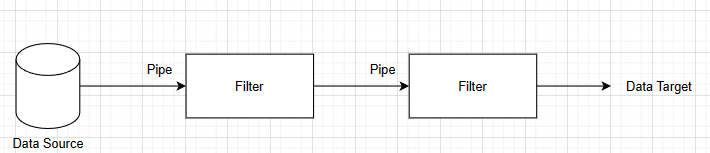
\includegraphics{Capture.png}
	Seperti yang Anda lihat pada diagram, data mengalir dalam satu arah. Ini dimulai dari sumber data, tiba di port input filter tempat pemrosesan dilakukan pada komponen, dan kemudian, diteruskan melalui port outputnya melalui pipa ke filter berikutnya, dan akhirnya berakhir di sasaran data.

	\section{Kelebihan}
	
	\begin{itemize}
		\item Memastikan sambungan komponen, filter yang longgar dan fleksibel.
		\item Kopling longgar memungkinkan filter diubah tanpa modifikasi ke filter lain.
		\item Konduktif untuk pemrosesan paralel.
		\item Filter dapat diperlakukan sebagai kotak hitam. Pengguna sistem tidak perlu mengetahui logika di balik kerja setiap filter.
		\item Dapat digunakan kembali. Setiap filter dapat dipanggil dan digunakan berulang kali.
	\end{itemize}
.
	
	
	\section{Kekurangan}
	
	\begin{itemize}
		\item 	Penambahan sejumlah besar filter independen dapat mengurangi kinerja karena overhead komputasi yang berlebihan.
		\item Bukan pilihan yang baik untuk sistem interaktif.
		\item Sistem pipa-dan-pemasang mungkin tidak cocok untuk perhitungan jangka panjang.
		
	\section{penerapan dalam aplikasi}
	\begin{itemize}
		\item Sistem pengolahan data: Pipe and filter dapat digunakan untuk mengambil data dari berbagai sumber dan memprosesnya melalui serangkaian filter untuk menghasilkan output yang diinginkan.
			
		\item Sistem pengolahan gambar: Pipe and filter dapat digunakan untuk memproses gambar atau video yang diambil dari kamera dengan menggunakan berbagai filter untuk menghasilkan gambar yang lebih baik atau memberikan efek khusus.
			
		\item Sistem pencarian: Pipe and filter dapat digunakan untuk memproses data pencarian yang diberikan oleh pengguna dan memfilter data untuk menghasilkan hasil pencarian yang relevan.
			
		\item Sistem pemrosesan audio: Pipe and filter dapat digunakan untuk memproses audio dan melakukan pengolahan suara seperti pengurangan kebisingan, pengaturan volume, dan pemotongan audio.
			
		\item Sistem pemrosesan teks: Pipe and filter dapat digunakan untuk memproses teks dan melakukan pengolahan bahasa alami seperti analisis sentimen dan pengenalan entitas.
			content...
		\end{itemize}
	\end{itemize}

